\documentclass[12pt]{article}
\usepackage[utf8]{inputenc}
\usepackage[margin=1in]{geometry}

\usepackage{biblatex}
\usepackage{indentfirst}
\usepackage{amsmath}
\usepackage{graphicx}
\usepackage{caption}
\usepackage{subcaption}

\graphicspath{ {images/} }

\renewcommand{\baselinestretch}{1.2}

\title{Discovering Panoramas in Web Videos}
\author{Lingfeng Huang, Fang Wang}

\date{11/2016}

\begin{document}
\maketitle

\section*{Abstract}
Panoramas have been widely used in may applications in multimedia, but the main constraint for panoramas is that they must be
taken by people who physically present at the place. In this project, we will implement our version of Discovering Panoramas in Web Videos by Liu et al. 
to solve the problem by selecting optimal segments within a given web videos, then perform synthesizing to obtain panoramas. This 
whole procedure is basically a optimization problem where we optimize the three criteria which are wide field of view, mosaicability, and high image 
quality.

\section{Introduction}
The emerge of the idea "Panorama" has to be dated back to early 20 A.D. and was a means of generating an 'panoptic' view of a vista \cite{wikipedia}. Nowadays, 
with the help of advancement of technology, people are able to create desired panorama by simply rotating their cell phones and clicking the shot button. The process
of synthesizing panorama is relatively straight forward. First step is to take successive photos from the same optical center and next step is finding the alignment between
each image and warping accordingly, and final step is interpolating the warped image and applied certain blending to remove the visible seams. However, the problem with creating
panoramas using above approach is that people are required to physically appear at the place where they take the images, which means that if people want to take a panorama
of Time Square in New York, they have to fly over New York to do so. \par
Compared to sequence of images, although some segments within videos have relatively low image quality and also moving object, they are still shot from the same optical center and cover a wide field-of-view. Lui et al. suggests an approach that synthesizing panoramas by identifying proper segments within videos as panorama source \cite{Lui}. They convert the problem into a optimization problem, and set up three constraints in order to evaluate the video segments. Lui ei al. indicates that in order to be a appropriate panorama source, a video segment should cover a wide field-of-view based on the definition of panorama imagery,  be "mosaicable" and the frames should have high image quality\cite{Lui}.

\section{Visual Quality Measure}
We measure the visual quality of a single frame based on two terms, one is incorrectness of the motion model $\mathit{E_{vm}(S_i)}$ and the source image visual quality $\mathit{E_{vv}(S_i)}$. Then by setting up the visual quality distortion $\mathit{E_v(S_i)}$, we can obtain the visual quality measure.
\begin{equation}
\mathit{E_v(S_i)} = \alpha_m\mathit{E_{vm}(S_i)} + \alpha_v\mathit{E_{vv}(S_i)}
\end{equation}
By default, we set both weights $\alpha_v$ and $\alpha_m$ to be 1.0.
\subsection{Source Image Visual Quality}
The source image visual Quality $\mathit{E_{vv}(S_i)}$ is defined as how blurry and blocky the image is. We use the idea of Tong et al.'s method of measuring blurring artifacts by using Haar Wavelet Transform \cite{Tong}.
\begin{figure}[htbp]
	\begin{subfigure}[b]{0.49 \textwidth}
	\centering
	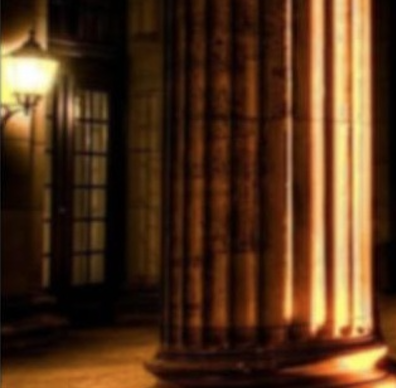
\includegraphics[width=7cm, height=7cm]{a}
	\caption{Blurriness: 0.8086}
	\label{default}
	\end{subfigure}
	%
	\hspace{1cm}
	%
	\begin{subfigure}[b]{0.49 \textwidth}
	\centering
	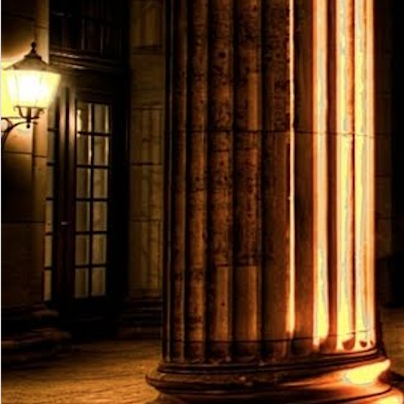
\includegraphics[width=7cm, height=7cm]{b}
	\caption{Blurriness: 0.3648}
	\label{default}
	\end{subfigure}
\caption{Blurriness measure compare}
\end{figure}
\par
The blockiness is measured by using the method of Wang et al. which estimates the average difference across block boundaries modulated by image activities \cite{Wang}.
\begin{figure}[h]
	\begin{subfigure}[h]{0.49 \textwidth}
	\centering
	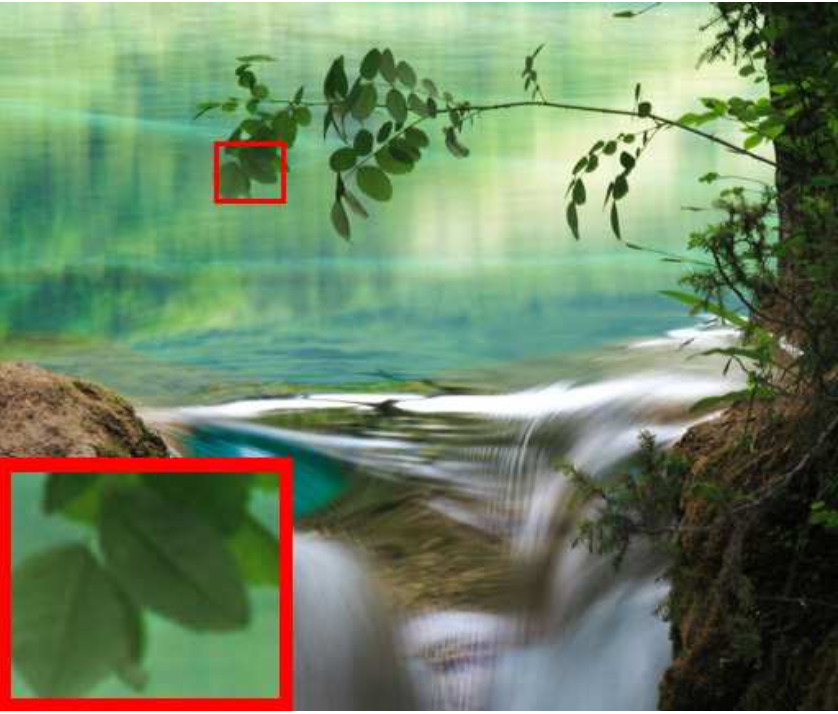
\includegraphics[width=7cm, height=7cm]{a1}
	\caption{Blockiness: 0.204}
	\label{default}
	\end{subfigure}
	%
	\hspace{1cm}
	%
	\begin{subfigure}[h]{0.49 \textwidth}
	\centering
	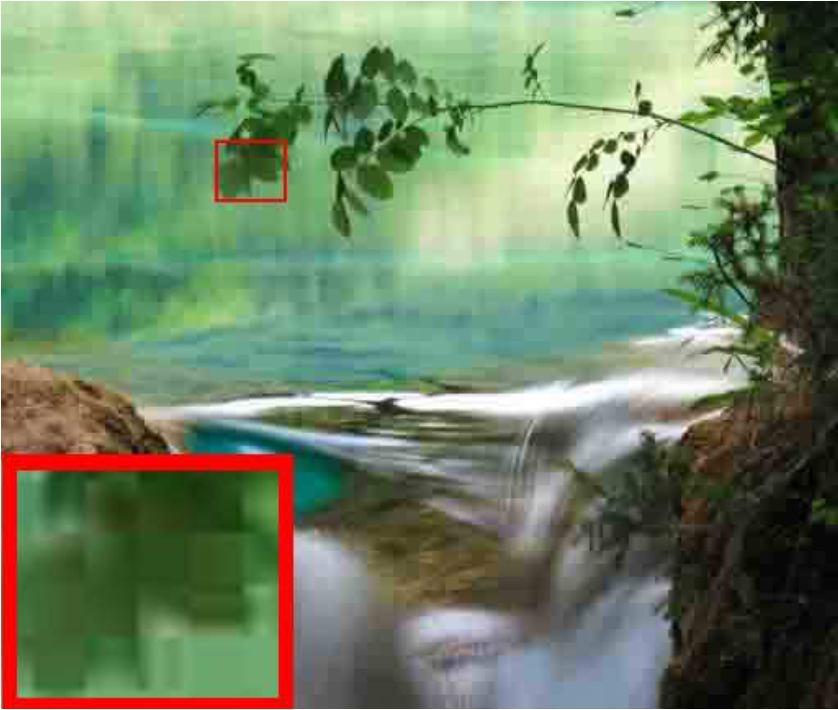
\includegraphics[width=7cm, height=7cm]{b1}
	\caption{Blockiness: 0.479}
	\label{default}
	\end{subfigure}
\caption{Blockiness measure compare}
\end{figure}

After obtain the blockiness and blurriness from all the frames within a given video segment, we calculate the visual distortion for this segment as follows:
\begin{equation}
\mathit{E_{vv}(S_i)} = \sum_{\substack{\mathit{I_k\in S_i}}}\gamma \mathit{q_{bk}(I_k)} + (1 - \gamma)\mathit{q_{br}(I_k)}
\end{equation} 
where $\mathit{q_{bk}(I_k)}$ is the measurement of blockiness of given frame, and $\mathit{q_{br}(I_k)}$ is the measurement of blurriness. Weight $\gamma$ is set to 0.45.

\subsection{Incorrectness of Motion Model}
In order to achieve the "mosaicablity", we use a homography to model the motion between frames. By matching SIFT feature points, we are able to locate significant points between frames and thus obtain the homography. In practice, getting a high quality panorama from video requires the inter-frame motion is closed to its homography and few casual videos can achieve that. Therefore, we measure the error using the real motion vector from SIFT feature points and the predicted value by homography between two successive frames.
\begin{equation}
\mathit{E_{vm}(S_i)} = \sum_{\substack{\mathit{I_k\in S_i}}} \frac{1}{\mathit{n_k}} \sum_{\substack{\mathit{p_{j,k}}\in \mathit{S_i}}} \lVert \mathit{mv(p_{j,k})}, \mathit{mv_h(p_{j,k})} \rVert
\end{equation}
We first for each adjacent frame $\mathit{I_k}$ and $\mathit{I_{k + 1}}$ find its matching SIFT feature pairs, and calculate homography using RANSAC based on these feature pairs. The notation $\mathit{mv(p_{j,k})}$ is the motion vector of $\mathit{j^{th}}$ SIFT feature point of frame $\mathit{I_k}$ and $\mathit{mv_h(p_{j,k})}$ is the predicted motion vector by homography at $\mathit{j^{th}}$ feature point. Then the error of $\mathit{j^{th}}$ feature point is taking the L1 norm of these two terms. Then we average the errors of all feature pair in each frame and obtain the incorrectness of motion model by summing up all the average. 
 
 \section{Extent of Scene}
 	The extent of scene $\varepsilon(\mathit{S_i})$ is defined as the scene covered by the video segment. Although it could be good if we maximizing the covering area to obtain a larger field of view, larger field of view often means more distortion. Hence, we want to choose the reference frame where the distortion is minimum, in other words, we want the minimum area covered by segment $\mathit{S_i}$
	
\begin{figure}[h]
	\centering
	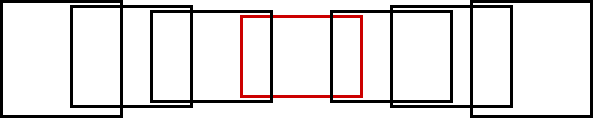
\includegraphics[width=15cm]{reference}
	\caption{All the other frames in the video are alignment to the reference frame, and we want to find the optimal reference frame so that the area covered by aligning all the frames to be minimized}
\end{figure}

In order to find the optimal reference frame, we want to search for all possible combination of panorama alignment as follows:
\begin{equation}
\mathit{r} = \mathrm{arg} \min_{\mathit{f_r} \in \mathit{S_i}} \bigcup_{\mathit{f} \in \mathit{S_i}} \mathit{I(f, f_r)}
\end{equation}
Then the extent of scene is defined as:
\begin{equation}
\varepsilon(\mathit{S_i}) = \bigcup_{\mathit{f} \in \mathit{S_i}} \mathit{I(f, r)}
\end{equation}
In Lui et al. paper, they used generic polygon clipping for finding the minimum area covered. However, we used another approach.  Although the accuracy declines, the complexity reduces in decent amount, we choose to find the distance between the center of reference frame and that of all other frames as follows:
\begin{equation}
\frac{1}{\mathit{n}} \sum_{\mathit{f \in S_i}}  \lVert \mathit{C_r}, \mathit{f_r} \rVert
\end{equation}
Where $\mathit{n}$ is the number of frames within the segment, $\mathit{C_r}$ is the center pixel of the reference frame and $\mathit{f_r}$ is the center pixel in a given frame.
\begin{figure}[h]
	\centering
		\begin{subfigure}{1\textwidth}
		\centering
			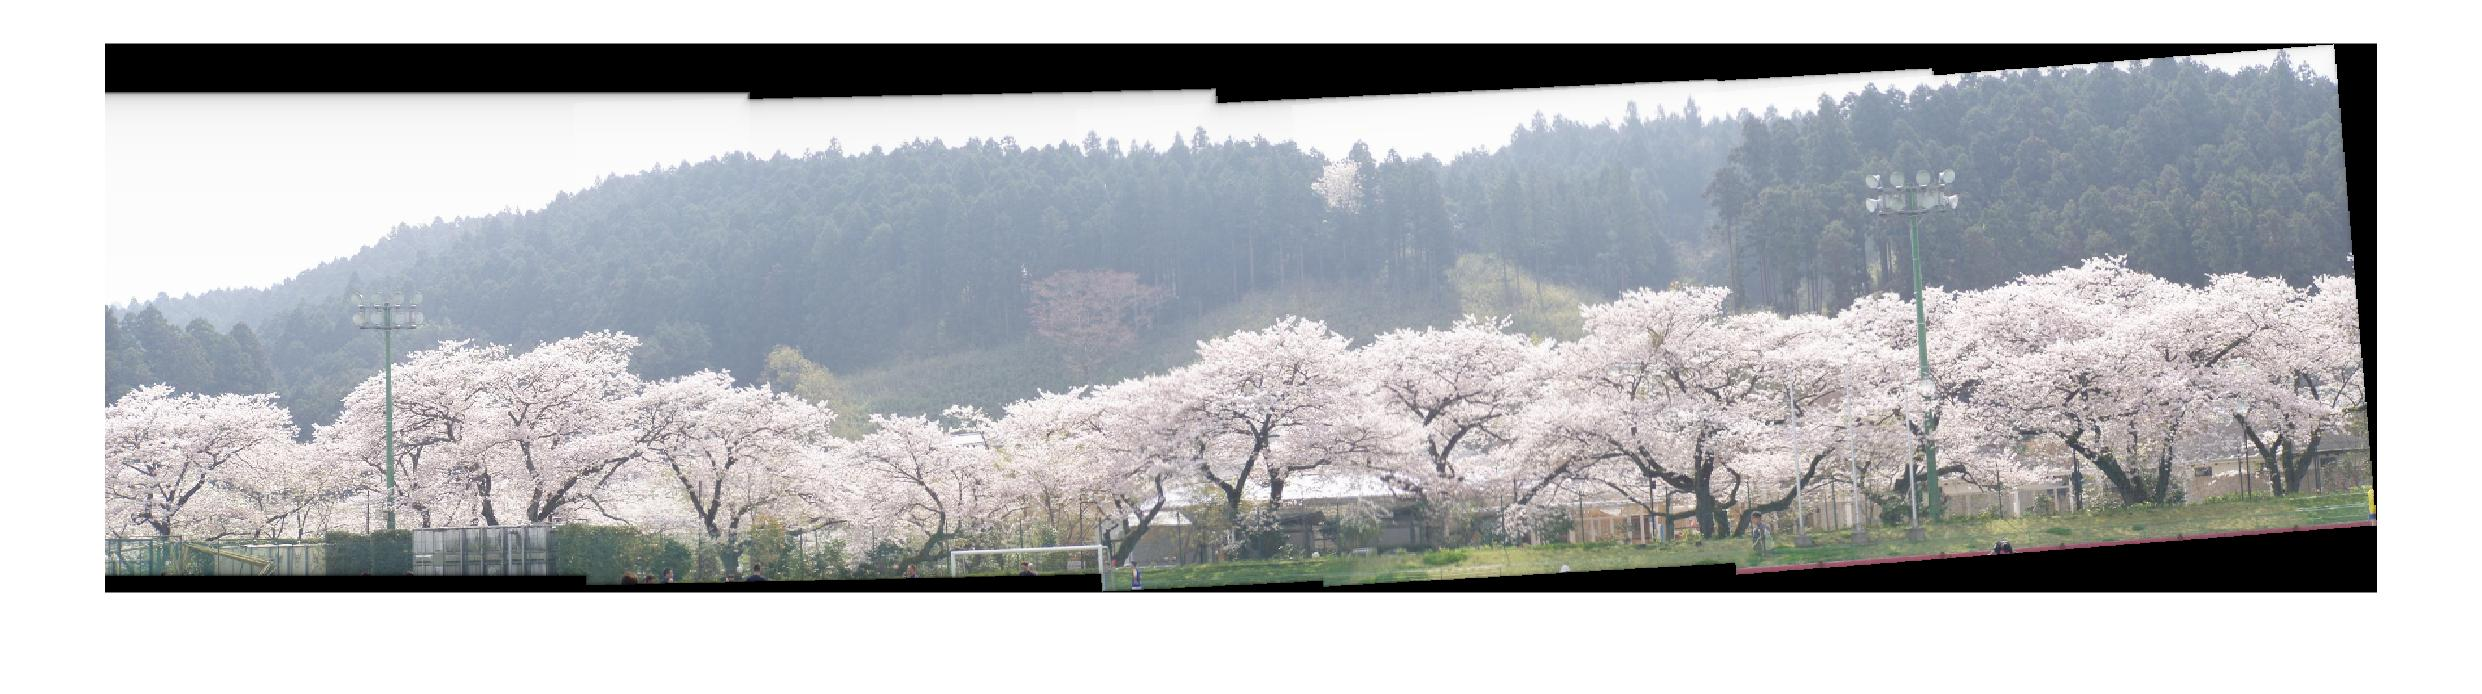
\includegraphics[height=3.5cm, width=15cm]{ref1}
			\caption{The reference frame is set at the left most frame}
			\label{fig:ref1}
		\end{subfigure}
		~
		\begin{subfigure}{1\textwidth}
		\centering
			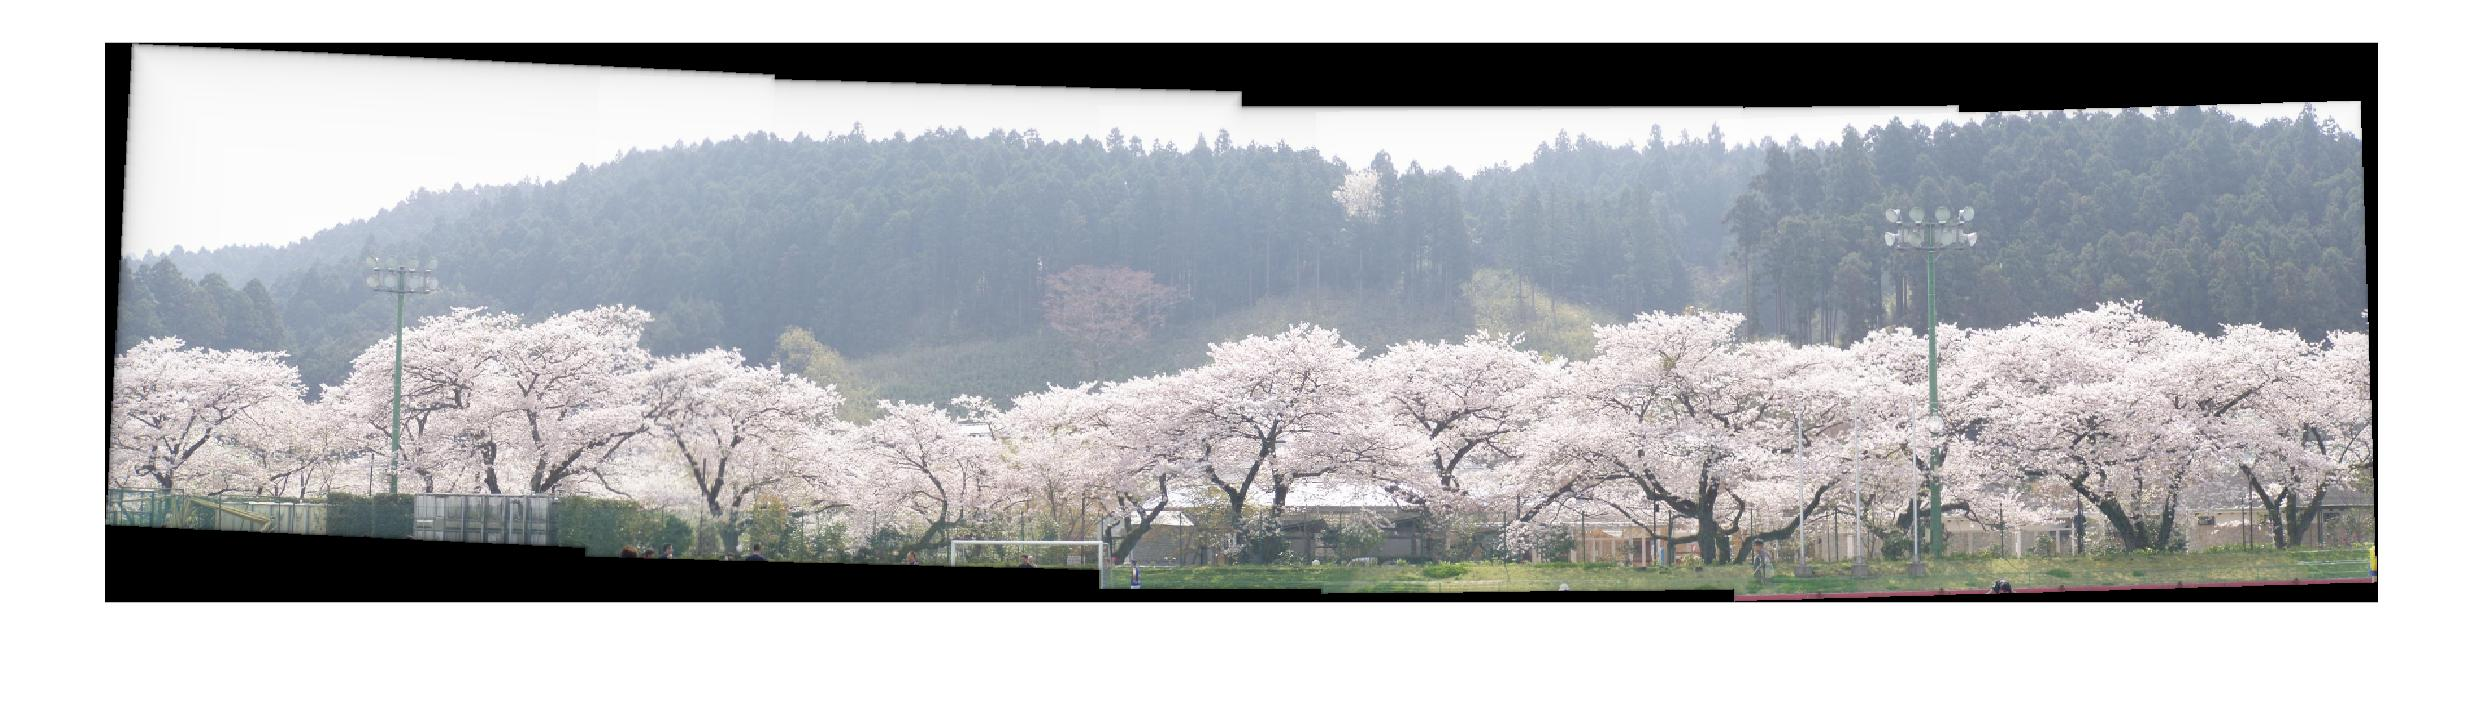
\includegraphics[height=3.5cm, width=15cm]{ref3}
			\caption{The reference frame is set at the center frame}
			\label{fig:ref3}
		\end{subfigure}
		~
				\begin{subfigure}{1\textwidth}
		\centering
			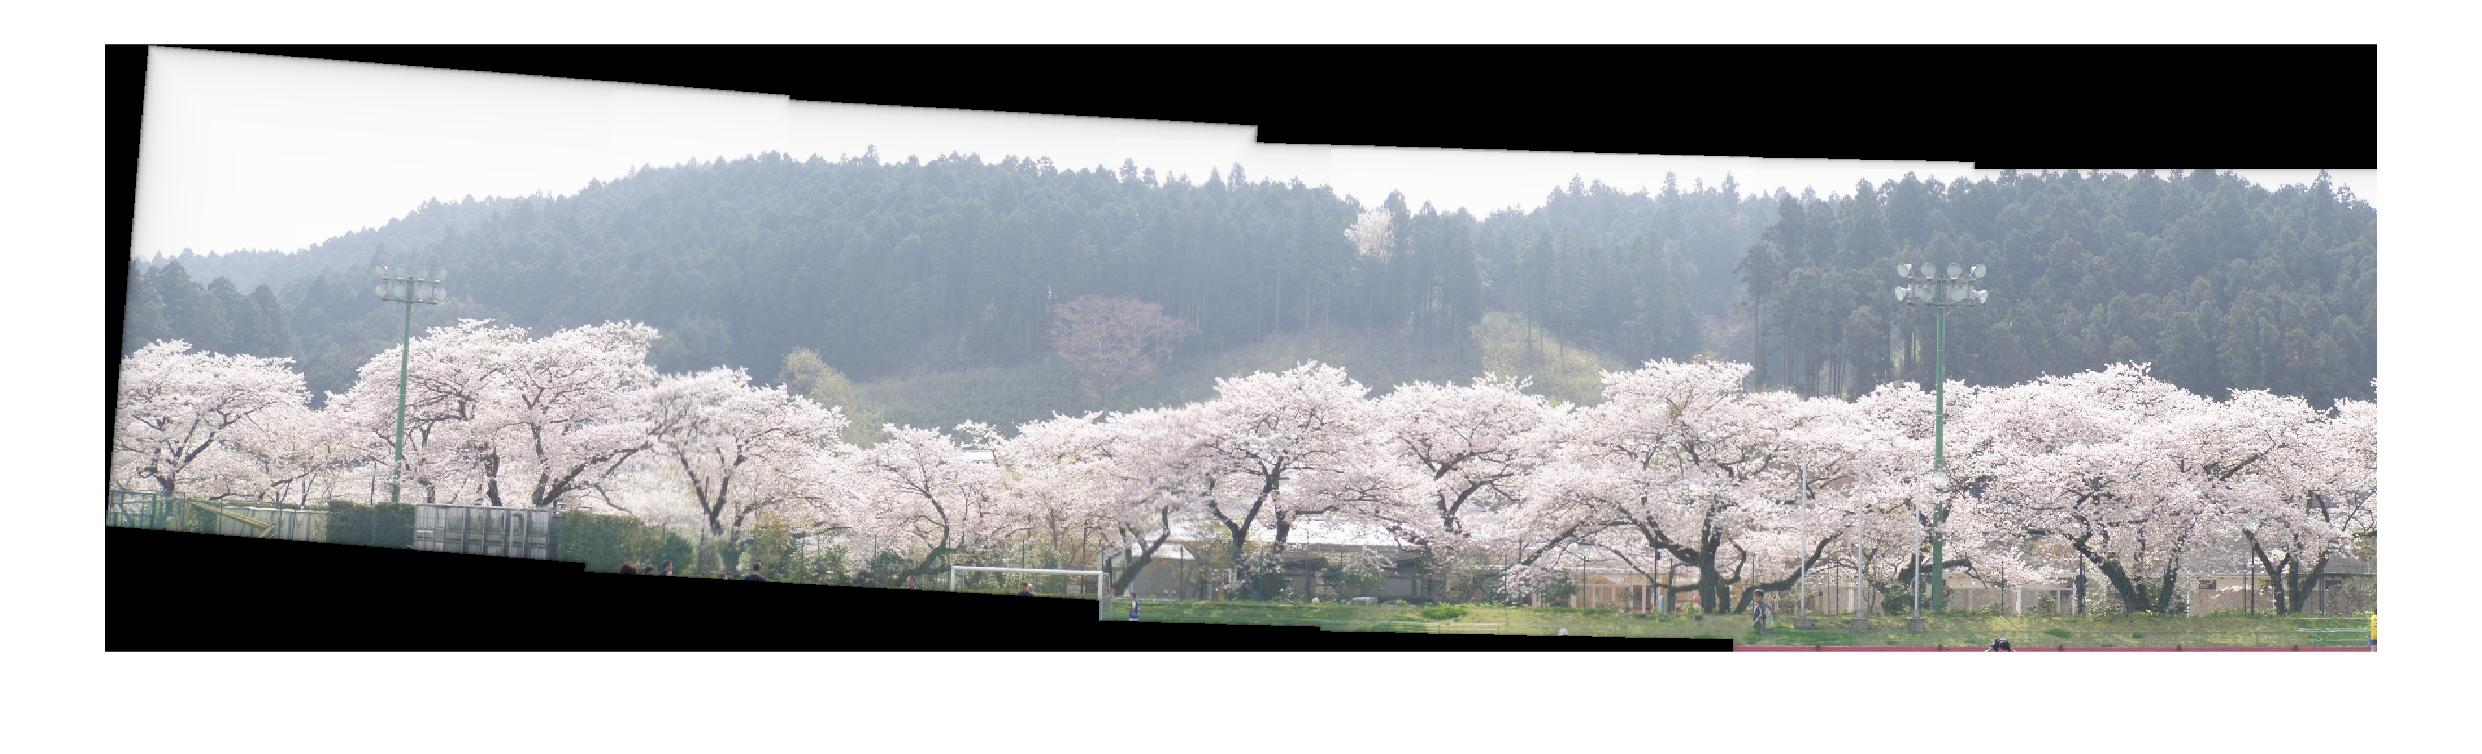
\includegraphics[height=3.5cm, width=15cm]{ref5}
			\caption{The reference frame is set at the right most frame}
			\label{fig:ref5}
		\end{subfigure}
		\caption{Difference reference frame results in different look of panorama}
\end{figure}
Figure 4 demonstrates when reference frame is the most left frame (the first frame in the image sequence), the middle frame and the right most frame. However, due to the relatively small distortion since this image sequence only has 5 images, the visual difference between three panoramas is subtle. 

\section{Experiments}
We randomly select some videos from Youtube and manually chop the video into several segments. Lui et al. use histogram based shot boundary detection to divide the video, and in order to simplify the process, we choose to feed our algorithm with preprocessed video segments.
\section{Limitations}
First of all, this whole process is not fully automated. At this point, we are not able to pass a whole video and get several possible results. Second, the complexity of this algorithm seems relatively high since we need to recalculate the homographies between adjacent frame for each iteration when we calculate the extent of scene. In addition, the run time for computing blurriness for each frame is also relatively high. 
\end{document}
